










\section{Abstract}


\tmpsection{One or two sentences providing a basic introduction to the field}
% comprehensible to a scientist in any discipline.
\lettr{A}n increasingly large fraction of emerging diseases come from wild animals and these diseases have a huge impact on human health, healthcare systems and economic development.
The chance that a new zoonosis will come from any particular wild host species increases with the diversity of pathogens in that species \cite{wolfe2000deforestation}.
However, the factors that control pathogen diversity in wild populations are still unclear.



\tmpsection{Two to three sentences of more detailed background}
% comprehensible to scientists in related disciplines.

% Add mechanistic vs empirical
Host species traits such as population density, longevity, body size and population structure have been shown to correlate with pathogen diversity.
Typically it is assumed that well-connected, unstructured populations promote the invasion of new pathogens and therefore increase pathogen diversity. % Where or how to define well-connected?
However, this assumption is largely untested; in particular our mechanistic understanding of how population structure affects pathogen diversity, in the presence of inter-pathogen competition, is poor.
Greater understanding is needed to clarify exactly by which mechanisms population structure affects pathogen diversity. 
%Mechanistic models are also likely to be more robust to transferring understanding between taxa and predicting changes. % !!! Not great.


%However, if competition is strong endemic pathogens will dominate and prevent new diseases from invading and spreading.
%In a structured population, stochastic effects could create areas of low prevalence of the endemic disease, allowing new diseases to invade.

\tmpsection{One sentence clearly stating the general problem (the gap)}
% being addressed by this particular study.
It is unknown whether population structure allows invading pathogens to escape from competition by stochastically creating areas of low pathogen prevalence.
I hypothesised that low dispersal rates and a low number of connections in a metapopulation network will allow invading pathogens to establish more readily, thus increasing pathogen diversity. 
I tested these hypothesese using population networks parameterised to mimic wild bat populations as bats have highly varied social structures and have recently been implicated in a number of high profile diseases such as Ebola, SARS, Hendra and Nipah.

\tmpsection{One sentence summarising the main result}
%  (with the words “here we show” or their equivalent).
I find that neither population connectedness nor dispersal rate affect the probability that a new pathogen will invade into a population.
%\paragraph{Two or three sentences explaining what the main result reveals in direct comparison to what was thought to be the case previously}
% or how the main result adds to previous knowledge
The assumption that factors causing high $R_0$ allow new pathogens to invade and therefore increase pathogen diversity is not supported.
Instead we find that changes in population structure do not affect the probability of invasion of a new pathogen.
 

\tmpsection{One or two sentences to put the results into a more general context.}
This result implies that population structure does not control pathogen diversity.
Instead it seems that local dynamics, that affect the short term branching process at the very start of the epidemic control the chance of pathogen invasion.
This also implies that population structure is not a useful proxy for pathogen diversity with respect to zoonotic disease surveillance, for example in bats.


%\tmpsection{Two or three sentences to provide a broader perspective, }
% readily comprehensible to a scientist in any discipline.





%%%%%%%%%%%%%%%%%%%%%%%%%%%%%%%%%%%%%%%%%%%%%%%%%%%%%%%%%%%%%%%%%%%%%%%%%%%%%%%%%%%%%%%%%%%%%%%%%%%%%%%%%%%%%%%%%%%%%%%%%%%%%%%%%%%%%%%%%%%%%%%%%%%%%%%%%%%


\section{Introduction}

%%%%%%%%%%%%%%%%%%%%%%%%%%%%%%%%%%%%%%%%%%%%%%%%%%%%%%%%%%%%%%%%%%%%%%%%%%%%%%%%%%%%%%%%%%%%%%%%%%%%%%%%%%%%%%%%%%%%%%%%%%%%%%%%%%%%%%%%%%%%%%%%%%%%%%%%%%%




\tmpsection{General Intro}
%%%%%%%%%%%%%%%%%%%%%%%%%%%%%%
% A basic introduction to the field,
% comprehensible to a scientist in any discipline.


\tmpsection{Why is pathogen diversity important?}
Over 50\% of emerging infectious diseases have an animal source \cite{jones2008global, smith2014global}.
Zoonotic pathogens can be highly virulent \cite{luby2009recurrent, lefebvre2014case} and potentially have huge public health impacts \cite{granich2015trends}, economic costs \cite{knobler2004learning} and slow down international development \cite{ebolaWorldbank}.
Therefore understanding and predicting changes in the process of zoonotic spillover is a global health priority \cite{taylor2001risk}.
The number of pathogen species hosted by a wild animal species affects the chance that a disease from that species will infect humans.
However, the factors that control the diversity of pathogens in a wild animal population are still unclear \cite{metcalf2015five}; in particular our mechanistic understanding of how population processes inhibit or promote pathogen richness is poor.



\tmpsection{Specific Intro}
%%%%%%%%%%%%%%%%%%%%%%%%%%%%%%
% more detailed background}
% comprehensible to scientists in related disciplines.


\tmpsection{We know some factors that correlate with pathogen diversity}
%population density, longevity, body size and population structure

A number of host traits have been shown to correlate with pathogen richness including body size \cite{kamiya2014determines, arneberg2002host}, population density \cite{nunn2003comparative, arneberg2002host} and range size \cite{bordes2011impact, kamiya2014determines}.
There are few studies that study population structure in a comparative framework.
Maganga \emph{et al.} found that distribution fragmentation predicts viral richness \cite{maganga2014bat}, but \cite{gay2014parasite} finds the opposite relationship. 
While the data set in \cite{gay2014parasite} is larger, the analysis in \cite{maganga2014bat} is much more focused on fragmentation.
Genetic correlates of population structure have also been used.
Turmelle \emph{et al.} \cite{turmelle2009correlates}, in a small analysis, find that high $F_{st}$ (i.e. a structured population) correlates with high richness.
However, they do not account for the widely different spatial scales found in population structure studies, nor do they deal with the differences between $F_{ST}$, $\phi_{ST}$ and other measures appropriately. 

Empirical, correlative studies are often contradictory due to small sample sizes, noisy data and because empirical relationships often do not extrapolate well to other taxa (though see \cite{kamiya2014determines} for a meta-analysis).
The correlation between many traits (e.g., \textcite{nunn2015infectious}) also makes it hard to clearly distinguish which factors are important.
Furthermore, knowing which factors correlate with pathogen richness does not tell us how they control richness. 
Mechanisms by which a trait could increase pathogen diversity include promoting the evolution of new strains within a species \cite{buckee2004effects}, reduction of the rate of pathogen extinction \cite{rand1995invasion} and an increased probability of pathogen invasion from other host species \cite{nunes2006localized}.
These separate mechanisms have not been examined and it is difficult to see how they could be approached through comparative methods.
We need explicit mechanistic models in order to tease apart these factors.
Furthermore, a solid mechanistic understanding of these processes will allow us to predict how wild populations will respond to increased human pressure and global change.
As habitats fragment we expect wild populations to become smaller and less well connected.
Understanding how these population changes interact reqiures a mechanistic understanding of disease dynamics.
Different specific mechanisms predict responses to climate change at different rates --- the extinction of parasites could occur relatively rapidly, whereas processes whereby invasive pathogens can persist more easily are likely to change pathogen community competition relatively slowly.

\tmpsection{Population structure could be important}



\tmpsection{Network structure has been studied}
 
% Analytical models
% +netCoex

Studies of the role of population structure on pathogen diversity have been in very simple systems.
These have been so simple that empirical data cannot easily be applied to them to predict pathogen diversity of real wild animal populations.
There is a need for models that can be carefully and fully explored, while still capturing the complexities of the real world.

In analytical models of well mixed populations competitive exclusion has been predicted \cite{ackleh2003competitive, bremermann1989competitive, martcheva2013competitive, qiu2013vector, allen2004sis}.
When competitive exclusion occurs, population structure has sometimes been shown to allow coexistence \cite{qiu2013vector, allen2004sis, nunes2006localized, garmer2016multistrain}.
Competing epidemics, or two pathogens spreading at the same time in a population, is a well studied area \cite{poletto2013host, poletto2015characterising, karrer2011competing}. 
This area is related to the study of pathogen richness in that they indicate that dynamics of multiple pathogens in a population do depend on population structure.
However, the results for short term epidemic competition do not directly transfer to the study of long term disease persistence which is the relative time scale when looking at zoonotic potential of a host species.


One commonly taken assumption in the ecological literature is that factors that promote high disease spread automatically promotes high diversity \cite{nunn2003comparative, morand2000wormy, poulin2014parasite, poulin2000diversity, altizer2003social}; this is contrary to the predictions from analytical models \cite{qiu2013vector, allen2004sis, nunes2006localized}. 
Furthermore, this assumption ignores competitive mechanisms such as cross-immunity and depletion of susceptible hosts.
If competitive mechanisms are strong, pathogens in populations structured such that $R_0$ will be high will be able to easily out-compete invading pathogens.
Only if competitive mechanisms are weak will high $R_0$  enable the invasion of new pathogens and allow higher pathogen diversity.

\tmpsection{Types of population structure}

How structured a population is can be defined in many ways on many scales.
Social group size is often examined as an indicator of population in large because the data are readily available.
However, group size is only one aspect of population structure.
Dispersal between is also a vital component of population structure.
Furthermore, many species exhibit fission-fusion social structures or other less clearly defined groupings.

The most relevant scale to study is that of an epidemiological population.
This is the population within which a pathogen can spread in an epidemiologically relevant time period (years or decades).
It is therefore closely related to a population as defined by population genetics, but with movement defined on a shorter time scale.

The epidemiological contacts within the population can be examined at the individual level (as in contact network epidemiology) or larger scales.
I consider the metapopulation network the most appropriate.
Ignoring the metapopulation assumes a fully mixed population which is unlikely.
Trying to study the contact network relies detailed individual level detail which is not available.
Metapopulation models consider a network of small subpopulations. 
Within subpopulations, epidemiological contacts are fully mixed and relatively fast.
Between subpopulations, epidemiological contacts are dependant on an underlying network structure and relatively slow.
The network underlying the metapopulation is made up of nodes representing the subpopulations, and edges which represent movement between subpopulations.
Animals, and therefore infection, can only move between two subpopulations if they are connected by an edge.

There are two factors that affect how structured a population is, given this model framework.
Firstly, dispersal is the rate at which individuals move between subpopulations.
Secondly, the metapopulation network structure controls population structure.
The simplest measure of how structured the network is the average number of edges each node has.
In the extremes, all subpopulations could be either connected to all other subpopulations or only connected to one or two other subpopulations.
However, other measures that take into account second-order structure in the network are also often used.





\tmpsection{The gap}
%%%%%%%%%%%%%%%%%%%%%%%%%%%%%%
% One sentence clearly stating the general problem
% being addressed by this particular study.
% By this stage, must have defined/introduced all terms used within.

Currently the literature contains very abstract, simplified models \cite{qiu2013vector, allen2004sis, nunes2006localized, garmer2016multistrain}.
These cannot be easily applied to real data.
They also do not easily quantitative predict pathogen pathogen; typically they predict either no pathogen coexistence \cite{bremermann1989competitive, martcheva2013competitive} or infinite pathogen diversity \cite{may1994superinfection}.
We need models that can give quantative predictions of pathogen richness in wild populations.
While predicting an absolute value of pathogen richness is likely to be impossible, we should aim for models that attempt to rank species from highest to lowest pathogen richness.
This requires a middle ground of model complexity.


To this end I have run metapopulation, multipathogen, epidemiological simulations based broadly on real-world bat populations.
Although still simplified, the model is complex enough that if good measurements of bat populations could be found, simulations of the real world bat population could be run.
Specifically I used these models to test the affects of population structure on the ability of a new pathogen to invade a population.
I tested two aspects of structure, dispersal rate and connectedness of the metapopulation network.


\tmpsection{Why bats}
I have used bats as a case study as they have an unusually large variety of social structures.
Colony sizes range from 10 to 1 million \cite{jones2009pantheria}.
Many bats also have interesting seasonal behaviour such as migration \cite{richter2008first, fleming2003ecology}, hibernation, birth puleses and swarming behaviours.
A number of traits have been suggested as predisposing bats towards being reservoirs of zoonotic diseases: high sympatry \cite{luis2013comparison}, flight \cite{wang2011mass}, longevity \cite{wang2011mass} as well as population structure \cite{maganga2014bat, turmelle2009correlates, gay2014parasite}.
Furthermore, bats have, over the last decade, become a focus for disease research  \cite{calisher2006bats, hughes2007emerging}.
Recently they have been implicated in a number of high profile diseases such as Ebola, SARS, Hendra and Nipah  \cite{calisher2006bats, li2005bats}.




\tmpsection{What I did}
%%%%%%%%%%%%%%%%%%%%%%%%%%%%%%

I have studied the invasion of new pathogens as a mechanisms for increasing pathogen richness.
I have studied two metrics for population structure, dispersal rate and metapopulation network topology, to test for effects of population structure on pathogen richness.
In particular I have focussed on studying the invasion of a newly evolved pathogen that is therefore identical in epidemiological parameters to the endemic pathogen.
Furthermore, this close evolutionary relationship means that cross immunity is strong.

\tmpsection{What I found}
%%%%%%%%%%%%%%%%%%%%%%%%%%%%%%
% One sentence summarising the main result
% (with the words “here we show” or their equivalent).

Here I show that, given the assumptions of a metapopulation, population structure does not affect the rate of invasion of new pathogens.
This is true whether population structure is altered by changing the dispersal rate or the topology of the metapopulation network.





%%%%%%%%%%%%%%%%%%%%%%%%%%%%%%%%%%%%%%%%%%%%%%%%%%%%%%%%%%%%%%%%%%%%%%%%%%%%%%%%%%%%%%%%%%%%%%%%%%%%%%%%%%%%%%%%%%%%%%%%%%%%%%%%%%%%%%%%%%%%%%%%%%%%%%%%%%%

\section{Methods}

%%%%%%%%%%%%%%%%%%%%%%%%%%%%%%%%%%%%%%%%%%%%%%%%%%%%%%%%%%%%%%%%%%%%%%%%%%%%%%%%%%%%%%%%%%%%%%%%%%%%%%%%%%%%%%%%%%%%%%%%%%%%%%%%%%%%%%%%%%%%%%%%%%%%%%%%%%%

%%

\begin{table}[b!]
\centering
\caption[All symbols used in Chapters \ref{ch:sims1} and \ref{ch:sims2}.]{All symbols used in Chapters \ref{ch:sims1} and \ref{ch:sims2} along with their units and default values.}

\begin{tabular}{@{}lp{5cm}p{3.9cm}r@{}}
\toprule
Symbol & Explanation & Units & Value\\
\midrule
$S$ & Number of susceptible individuals &&\\
$I_q$ & N. individuals infectious with diseases $q$ &&\\
$I^+_p$ & Sum of classes infected with pathogen $p$ &\\
$R$ & Number of recovered/immune individuals &&\\
$N$ & Total Population && 30,000\\
$m$ & Number of colonies&& 10\\
$n$ & Colony starting size && 3,000\\
$a$ & Area & km$^2$& 10,000\\
$\beta$ & Transmission rate & Per year per individual& 2, 5, 10\\
$\gamma$ & Recovery rate & Per year per individual. & 1\\
$\lambda$ & Dispersal & Per day per individual& 0.001--0.1\\
$\Lambda$ & Birth rate & Per year per individual& 0.05\\
$\mu$ & Death rate & Per year per individual & 0.05\\
%$d_I$ & Infectious death rate & Additional deaths per day per individual&\\
$\rho$ & No. pathogens && 2\\
$p$ &  Pathogen index i.e. $p\in\{1,2\}$ for pathogens 1 and 2 & &\\
$q$ & Disease class i.e., $q\in\{1,2,12\}$&\\
%$\mathcal{V}$ & Neighbourhood of a node &&\\
$t, t^\prime$ & Time and time plus waiting time i.e., $t+\delta$ & Days&\\
$k_i$ & Degree of node $i$ &&\\
$\delta$ & Waiting time until next event & Days&\\
$\alpha$ & Cross immunity & Proportion& 0.1\\
$n, m$ & Colony index &&\\
%$\bm{A}_{mn}$ & Adjacency matrix. & Distance &\\
%$\mu$ & Maximum distance for edge to exist & km& 40, 100\\
$\sigma$ & Invading pathogen seed size & & 10\\
$r_i$ & The rate that event $i$ occurs. & Days$^{-1}$&\\
\bottomrule
\end{tabular}

\label{t:params}
\end{table}




\subsection{Metapopulation model}




\paragraph{Two pathogen SIR model}

I examine a multipathogen SIR model with vital dynamics. 
This is a compartment model with individuals being classed as susceptible, infected or recovered with immunity (Figure~\ref{f:sir}).
Susceptible individuals are counted in class $S$.
There are three infected classes, $I_1$, $I_2$ and $I_{12}$, being individuals infected with pathogen 1, pathogen 2 or both respectively.
Recovered individuals, $R$, are immune to both pathogens, even if they have only been infected with one.
Furthermore, recovery from one pathogen moves an individual straight into the recovered class, even if the individual is infected with both pathogen.
This modelling choice allows the model to be easily expanded to include more than two pathogens.
The assumption of immediate recovery from all other diseases is likely to be quite accurate for very closely related pathogens as is being studied here as once an acquired immune response is activated, all infections are likely to be cleared quickly.

The coinfection rate (the rate at which an infected individual is infected with a second pathogen) is adjusted compared to the infection rate by a factor $\alpha$ (here I used $\alpha = 0.1$ which means coinfection happens at a tenth the rate of first infections).
In the application of long term existence of pathogens it is vital to include vital dynamics (births and deaths) as the SIR without vital dynamics has no endemic state.
Birth and death rates are assumed to be equal, $\mu = \Lambda$ (see Table~\ref{t:params} for a list of symbols and values used).
The time scale of the simulations are set by setting $\mu$ = 0.05 per year, yielding an average host generation time of 20 years.
Infection is assumed to cause no extra mortality as for a number of viruses, bats show no clinical signs of infection \cite{halpin2011pteropid, deThoisy2016bioecological}.


\paragraph{Metapopulation}


The population is divided into a number of subpopulations.
This metapopulation is modelled as a network with subpopulations being nodes and dispersal between subpopulations being indicated by edges (Figure~\ref{f:net}).
Individuals within a subpopulation interact randomly so that the subpopulation is fully mixed.
Dispersal between subpopulations occurs at a rate $\lambda$.
Individuals can only disperse to subpopulations connected to theirs in the network.
The rate of dispersal is not affected by the number of edges a subpopulation has (the degree of the subpopulation).
So the dispersal rate from a subpopulation $m$ with degree $k_m$ to subpopulation $n$ is $\frac{\lambda}{k_m}$.
Note this rate is independent of the degree of subpopulation $n$.





\paragraph{Stochastic simulations}

I examine this model using stochastic, continuous time simulations (using the Gillespie algorithm) implemented in R \cite{R}.
At each step in the simulation we calculate the rate that each possible event might occur.
One event is then randomly chosen, weighted by its rate
\begin{align}
  p(\text{event } i) = \frac{r_i}{\sum_i r_i}
\end{align}
where $r_i$ is the rate that event $i$ occurs.
Finally, the length of the time step, $\delta$, is drawn from an exponential distribution 
\begin{align}
  \delta \sim \operatorname{Exp}\left(\sum_i r_i  \right).
\end{align}
This means that the total length of each simulation is stochastic. 
We define the number of events we wish to simulate instead.


\begin{figure}[t]
\centering
  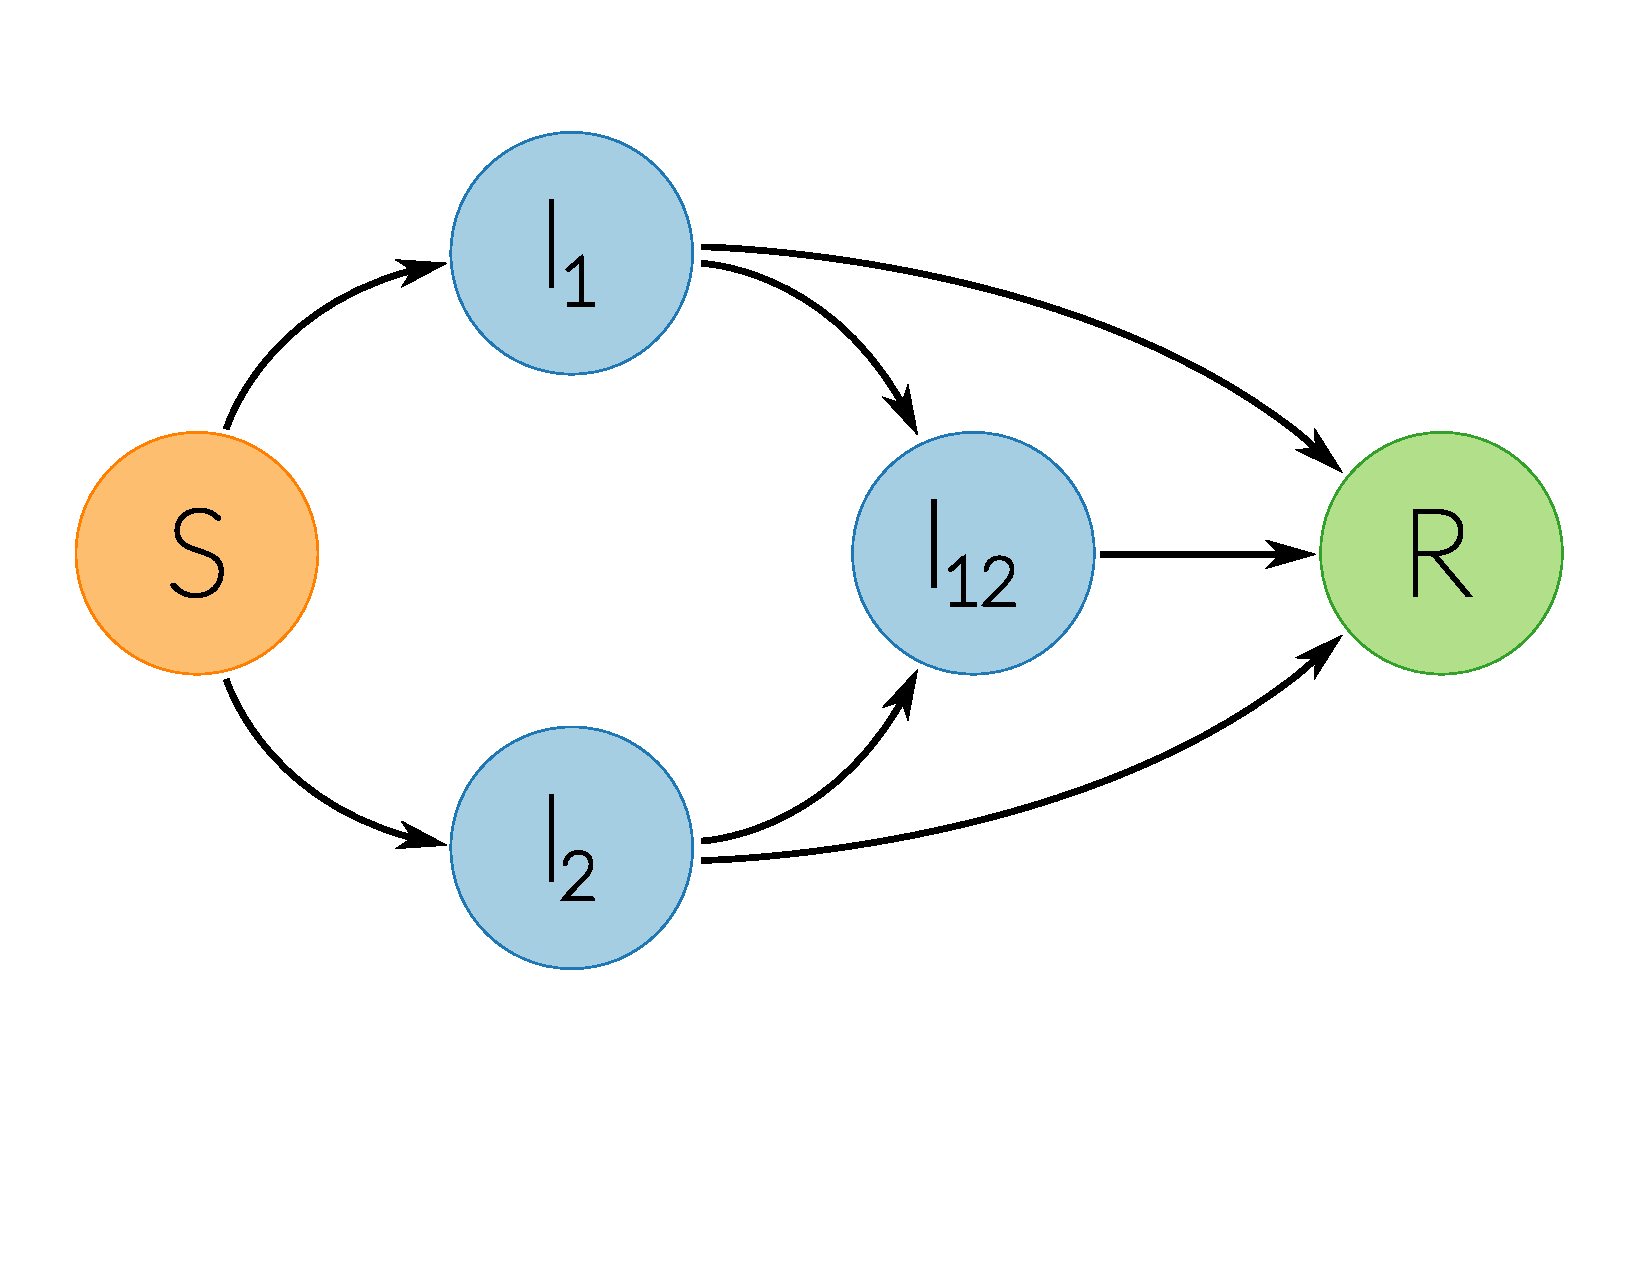
\includegraphics[width=0.4\textwidth]{imgs/SIRoption1.pdf}
  \caption[Schematic of the SIR model used]{
Schematic of the SIR model used. 
Individuals are in one five classes, susceptible (orange, S), infectious with pathogen 1, pathogen 2 or both (blue, $I_1, I_2, I_{12}$) or recovered and immune from further infection (green, R).
Transitions between classes occurs only as indicated by arrows.
Note that individuals in $I_{12}$ move into R, not back to $I_1$ or $I_2$. 
That is, recovery from one pathogen causes immediate recovery from the other pathogen.
}
  \label{f:sir}
\end{figure}


We can now write down the rates of all events. 
I defined $I^+_p$ to be the sum of all classes that are infectious with pathogen $p$, for example $I^+_1 = I_1 + I_{12}$. 
Assuming asexual reproduction, that all classes reproduce at the same rate and that individuals are born into the susceptible class we get
\begin{align}
  P\left( S_{nt^\prime} = S_{nt} +1\right) &= \Lambda\left( S_{nt}+\sum_q I_{qnt} + R_{nt}\right) 
\end{align}
where $P\left( S_{nt^\prime} = S_{nt} +1\right)$ is the probability that the number of susceptibles in subpopulation $n$ will increase by 1 (a single birth) in the time interval $t$ to $t^\prime$ and $\sum_q I_{qnt}$ is the sum of all infection classes $q \in {1, 2, 12}$.
The rates of death, given a death rate $d$ are given by
\begin{align}
  P\left( S_{nt^\prime} = S_{nt}-1 \right) &= \mu S_{nt}, \\
  P\left( I_{qnt^\prime} = I_{qnt}-1 \right) &= \mu I_{qnt},\\
  P\left( R_{nt^\prime} = R_{nt}-1 \right) &= \mu R_{nt}.
\end{align}
I modelled transmission as density-dependant.
This assumption was more suitable than frequency-dependant transmission as I am modelling a disease transmitted by saliva or urine in highly dense populations confined to caves, building or potentially a small number of tree roosts.
I was notably not modelling an STD as these diseases are not expected to be commonly zoonotic.
Infection of a susceptible with either pathogen 1 or 2, $S \rightarrow I_p$ where $p\in \{1,2\}$, is therefore given by
\begin{align}
  P\left( I_{pnt^\prime} = I_{pnt}+1, S_{nt^\prime} = S_{nt}-1 \right) &= \beta S_{nt}I^+_{pnt},
\end{align}
while coinfection, given a crossimmunity factor $\alpha$, is given by
\begin{align}
  P\left( I_{12,nt^\prime} = I_{12,nt}+1,\: I_{1nt^\prime} = I_{1nt}-1\right) = &\alpha\beta I_{1nt}I^+_{2nt},\\
  P\left( I_{12,nt^\prime} = I_{12,nt}+1,\: I_{2nt^\prime} = I_{2nt}-1\right) = &\alpha\beta I_{2nt}I^+_{1nt}.
\end{align}
The probability of migration from colony $m$ (with degree $k_m$) to colony $n$, given a dispersal rate $\lambda$ is given by
\begin{align}
  P\left(S_{nt^\prime}=S_{nt}+1,\: S_{mt^\prime} = S_{mt}-1\right) &= \frac{\lambda S_{mt}}{k_m-1},\\
  P\left(I_{qnt^\prime}=I_{qnt}+1,\: I_{qmt^\prime} = I_{qmt}-1\right) &= \frac{\lambda I_{qmt}}{k_m-1},\\
  P\left(R_{nt^\prime}=S_{nt}+1,\: R_{mt^\prime} = R_{mt}-1\right) &= \frac{\lambda R_{mt}}{k_m-1}.
\end{align}
Finally, recovery from any infectious class occurs at a rate $\gamma$
\begin{align}
  P\left( I_{qnt^\prime} = I_{qnt}-1,\: R_{nt^\prime} = R_{nt}+1 \right) &= \gamma I_{qnt}.
\end{align}


\begin{figure}[t]
{\centering 
\subfloat[Fully connected\label{fig:fullyConnected}]{
  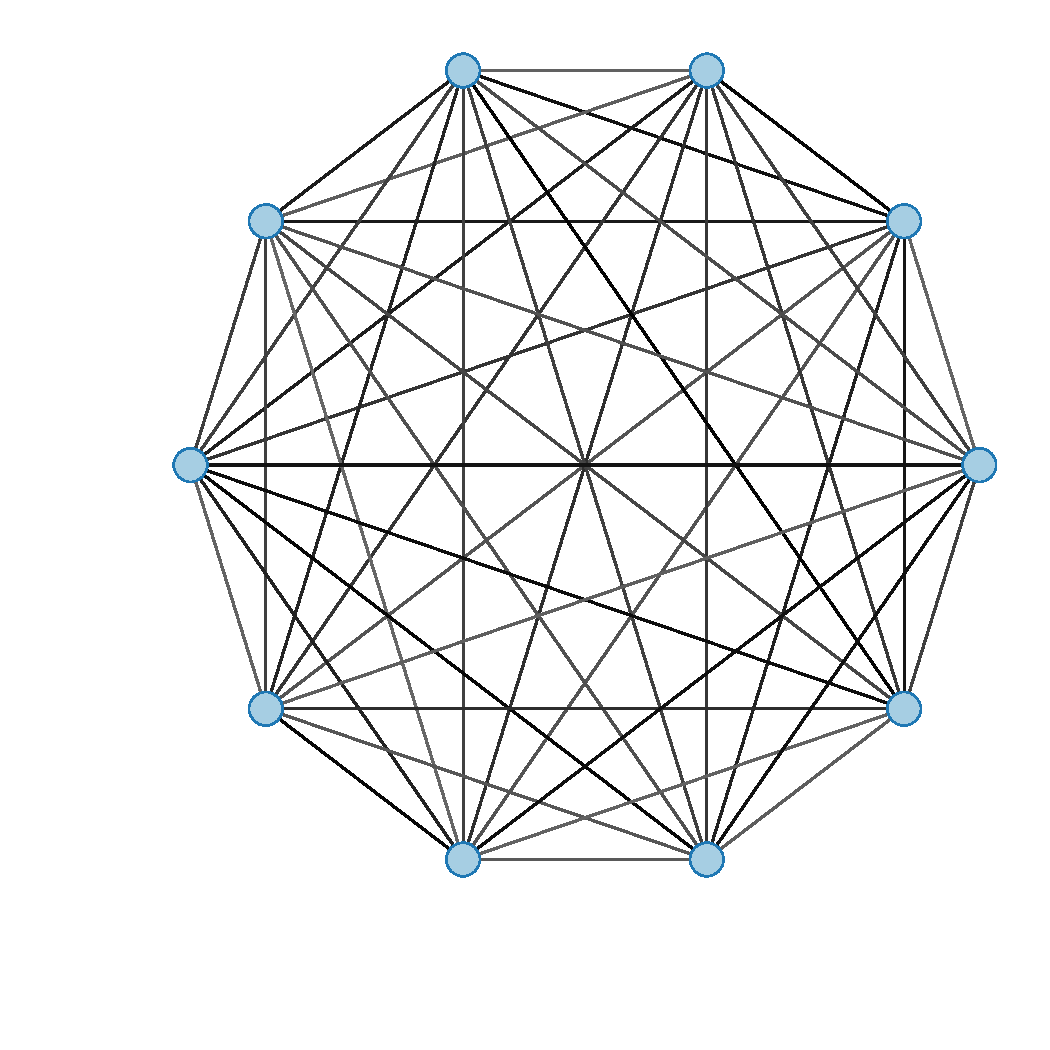
\includegraphics[width=0.45\textwidth]{imgs/fullyConnected.pdf} 
}
\subfloat[Minimally connected
\label{fig:minimallyConnected}]{
  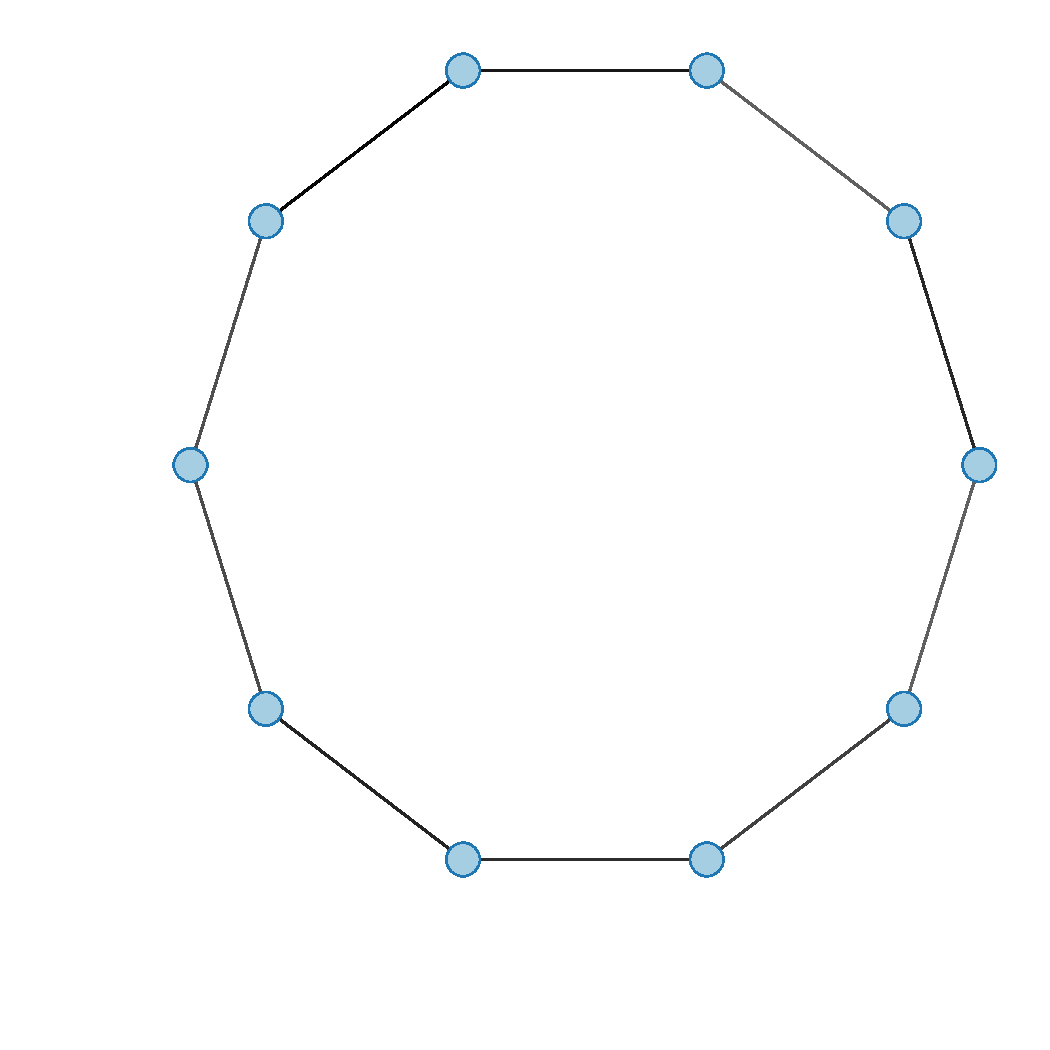
\includegraphics[width=0.45\textwidth]{imgs/minimallyConnected.pdf} 
}
}
\caption[Network topologies used to compare network connectedness]{
The two network topologies used to test whether network connectedness influences a pathogens ability to invade.
Blue circles are subpopulations of 3,000 individuals.
Dispersal only occurs between subpopulations connected by an edge (black line).
The dispersal rate is held constant between the two topologies.
A) Dispersal can occur between any subpopulation.
B) Animals can only disperse to neighbouring subpopulations. 
}
\label{f:net}
\end{figure}















In each simulation the population was seeded with 10 sets of 200 infected individuals of pathogen 1.
These groups were seeded into randomly selected colonies with replacement.
For each 200 infected individuals added, 200 susceptible individuals were removed to keep starting colony sizes constant. 
Pathogen 1 was then allowed to spread and reach equilibrium. 
After \ensuremath{3\times 10^{5}} events, 5 individuals infected with pathogen 2 were added to one randomly selected colony. 
Visual inspection of preliminary simulations was used to decide on \ensuremath{3\times 10^{5}} as being long enough for the epidemic to reach an equilibrium state.
After another \ensuremath{5\times 10^{5}} events the invasion of pathgen 2 was considered successful if any individuals are still infected with pathogen 2.
Again visual inspection of preliminary simulations was used to determine that after \ensuremath{5\times 10^{5}} events, if an invading pathogen was still present, it was well established. 


\subsection{Dispersal}
%%%%%%%%%%%%%%%%%%%%%%%%%%%%%%

The values used for the independant variables are chosen to highlight the affects of these variables. 
Dispersal values are $\lambda = 0.1, 0.01$ and $ 0.001$ dispersals per individual per year. 
$\lambda = 0.1$ relates to individuals moving between colonies on average twice per lifetime. 
Therefore exclusively juvenile dispersal would have dispersal rates similar to this. 
Otherwise it relates to dispersal being a rare event with animals often staying in a colony for many years.
$\lambda = 0.01$ relates to 20\% of individuals dispersing once in their lifetime.
This value is therefore close to male-biased dispersal, with female philopatry. 
Finally, $\lambda = 0.001$ relates to 2\% of individuals dispersing in their lifetime.
This therefore relates to a population that does not habitually disperse.




\subsection{Network structure}
%%%%%%%%%%%%%%%%%%%%%%%%%%%%%%
The network structure was synthetically created to be either fully or minimally connected (See Figure~\ref{f:net}). 
10 subpopulations was selected as a trade off between computation time and a network complicated enough that structure might have an effect. 
This value is artificially small compared to wildlife populations. 



\subsection{Parameter selection}


The fixed parameters used are chosen to roughly reflect realistic wild bat populations. 
The death rate $\mu$ was set as 0.05 per year giving a generation time of 20 years.
The birth rate $\Lambda$ was set to be equal to $\mu$ so that the population size was stable.
The recovery rate $\gamma$ was set to 1 giving a average infection duration of 1 years. 
This is therefore a long lasting infection but not a chronic infection. 
It is very difficult to directly estimate infection durations in wild populations but it seems that these infections might sometimes be long lasting \cite{peel2012henipavirus, plowright2015ecological}.
However, other studies have found much shorter infectious periods \cite{amengual2007temporal}.
These shorter lived in infections are studied further here as preliminary simulations found that they could not persist in the relatively small populations being modelled here.

Cross immunity was set to 0.1 so that an individual infected with one pathogen is 90\% less likely to be infected with another.
This is a rather arbitrary value.
However, the rationale of the model was that the invading species might be a newly speciated strain of the endemic species.
Furthermore, the model assumes complete cross immunity after recovery from infection.
Therefore cross immunity to coinfection is likely to be very strong as well.

The population size of each subpopulation was set to 3,000. 
This is appropriate for many bat species \cite{jones2009pantheria}, especially the large, frugivorous \emph{Pteropodidae} that have been particularly associated with recent zoonotic diseases.


Four values of the transmission rate $\beta$ are used, 0.1, 0.2, 0.3 and 0.4.
All simulations are run under all four transmission rates as this is such a fundamental parameter.
%Given the recovery, birth and death rates we can calculate an approximation of $R_0$ that ignores spatial structure.
%That is, this is $R_0$ for the local, within-subpopulation dynamics.
%Furthermore, it is $R_0$ for the first pathogen; $R_0$ of the invading pathogen will be lower due to competition.
%We can calculate that $R_0 \approx \frac{\beta b}{d(d+ \gamma)}$.
%For our four values of $\beta = 0.1, 0.2, 0.3, 0.4$ we therefore get $R_0 \approx 2.9, 4.8, 6.7, 8.6$.
%These values are very high in part to again find a reasonable trade off between the number of simulations and the reasonableness of the parameters.
%$R_0 \approx 13.3$ is similar to a highly contagious pathogen such as measles or pertussis. 

% R_\ast (R_0 - 1)\frac{\langle k^2 \rangle - \langle k \rangle}{\langle k^2 \rangle} \frac{p\bar{N}\alpha}{\mu} > 1
% N = avg pop size, p = migration, mu = recovery, \alpha N_k is number of individuals infected. So think this is not with vital dynamics.




%%%%%%%%%%%%%%%%%%%%%%%%%%%%%%%%%%%%%%%%%%%%%%%%%%%%%%%%%%%%%%%%%%%%%%%%%%%%%%%%%%%%%%%%%%%%%%%%%%%%%%%%%%%%%%%%%%%%%%%%%%%%%%%%%%%%%%%%%%%%%%%%%%%%%%%%%%%


\section{Results}

%%%%%%%%%%%%%%%%%%%%%%%%%%%%%%%%%%%%%%%%%%%%%%%%%%%%%%%%%%%%%%%%%%%%%%%%%%%%%%%%%%%%%%%%%%%%%%%%%%%%%%%%%%%%%%%%%%%%%%%%%%%%%%%%%%%%%%%%%%%%%%%%%%%%%%%%%%%








































\subsection{Invasion}


\paragraph{Dispersal}
%%%%%%%%%%%%%%%%%%%%%%%%%%%%%%


The proportion of invasions was not different across dispersal rates across 1200 simulations run (Figure \ref{f:invasionPropPlots}A).
This was true at all transmission levels ($\chi^2$ test. $\beta = 0.1$: $\chi^2 = 1.98$, $\text{df} = 2$, $p = 0.37$. $\beta = 0.2$: $\chi^2 = 9.44$, $\text{df} = 2$, $p = \ensuremath{8.9\times 10^{-3}}$. $\beta = 0.3$: $\chi^2 = 0.29$, $\text{df} = 2$, $p = 0.87$, $\beta = 0.4$: $\chi^2 = 0.83$, $\text{df} = 2$, $p = 0.66$).


\paragraph{Network structure}
%%%%%%%%%%%%%%%%%%%%%%%%%%%%%%

I ran 800 simulations over 4 transmission values ($\beta = $ 0.1, 0.2, 0.3, 0.4).
The proportion of invasions was not different between highly connected and largely unconnected metapopulations (Figure~\ref{f:invasionPropPlots}B). 
This was true at all transmission levels ($\chi^2$ test. $\beta = 0.1$: $\chi^2 < 10^{-5}$, $\text{df} = 1$, $p > 0.9999$. $\beta = 0.2$: $\chi^2 = 0.02$, $\text{df} = 1$, $p = 0.88$. $\beta = 0.3$: $\chi^2 = 1.53$, $\text{df} = 1$, $p = 0.22$. $\beta = 0.4$: $\chi^2 = 0.26$, $\text{df} = 1$, $p = 0.61$).

 
\subsection{Transmission}
%%%%%%%%%%%%%%%%%%%%%%%%%%

Inline with theory, increasing the transmission rate increased the probability of invasion (Figure~\ref{f:invasionPropPlots}).
This is true for all three dispersal values ($\chi^2$ test. $\lambda = 0.001$: $\chi^2 = 243.56$, $\text{df} = 3$, $p < 10^{-5}$. $\lambda = 0.01$: $\chi^2 = 265.4$, $\text{df} = 3$, $p < 10^{-5}$. $\lambda = 0.1$: $\chi^2 = 244.95$, $\text{df} = 3$, $p < 10^{-5}$) and both network structures ($\chi^2$ test. Fully connected: $\chi^2 = 267.3$, $\text{df} = 3$, $p < 10^{-5}$. Minimally connected: $\chi^2 =  267.3$, $\text{df} = 3$, $p < 10^{-5}$).









\begin{knitrout}\footnotesize
\definecolor{shadecolor}{rgb}{0.969, 0.969, 0.969}\color{fgcolor}\begin{figure}[t]

{\centering 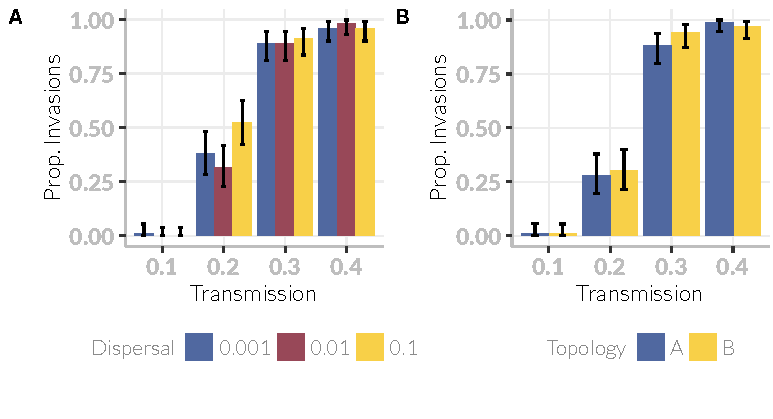
\includegraphics[width=\textwidth]{figure/invasionPropPlots-1} 

}

\caption[The probability of invasion across different dispersal rates and network topologies.]{The probability of successful invasion. 
  For three different transmission rates, the probability of invasion does not change between different a) dispersal rates or b) network topologies (with network topologies A and B refering to the    fully and minimally connected topologies in Figure~\ref{f:net}). 
  Error bars are 95\% confidence intervals. 
  100 simulations were run for each treatment.
  Other parameters are kept constant at: $N = 10,\, \, b = d = 0.05,\, \gamma = 0.1,\, \alpha = 0.1$. 
  When dispersal is varied, the population structure is fully connected. When population structure is varied, $\lambda = 0.01$.}\label{f:invasionPropPlots}
\end{figure}


\end{knitrout}




%%%%%%%%%%%%%%%%%%%%%%%%%%%%%%%%%%%%%%%%%%%%%%%%%%%%%%%%%%%%%%%%%%%%%%%%%%%%%%%%%%%%%%%%%%%%%%%%%%%%%%%%%%%%%%%%%%%%%%%%%%%%%%%%%%%%%%%%%%%%%%%%%%%%%%%%%%%


\section{Discussion}

%%%%%%%%%%%%%%%%%%%%%%%%%%%%%%%%%%%%%%%%%%%%%%%%%%%%%%%%%%%%%%%%%%%%%%%%%%%%%%%%%%%%%%%%%%%%%%%%%%%%%%%%%%%%%%%%%%%%%%%%%%%%%%%%%%%%%%%%%%%%%%%%%%%%%%%%%%%

\tmpsection{Restate the gap and the main result}

Empirical studies on the role of population structure on pathogen richness are equivocal and cannot examine the specific mechanisms by which pathogen communities are created and maintained.
I have used mechanistic, metapopulation models to test whether increased population structure can promote pathogen richness by facilitating invasion of new pathogens.
I find that population structure does not affect the ability of a new pathogen to invade and persist in a population.
Instead I find that only transmission rate affects the chance of pathogen invasion.
That population structure does not affect pathogen richness goes against many predictions that increasing $R_0$ increases pathogen richness \cite{nunn2003comparative, morand2000wormy, poulin2014parasite, poulin2000diversity, altizer2003social}.
However, simple analytical models suggest that population structure should increase pathogen richness \cite{qiu2013vector, allen2004sis, nunes2006localized} and I find no evidence of this either.

I have found no evidence that population structure aids the invasion and establishment of newly evolved pathogen species.
Instead it seems that invasion relies solely on the local dynamics of the disease.
If the transmission rate is high, a pathogen has a good chance of spreading immediately after its introduction when it is at low density.
Once the pathogen has infected a large number of individuals in the local metapopulation, it is bound to spread throughout the metapopulation without going extinct.

\tmpsection{Link results to consequences}

These results imply that if population structure does in fact affect pathogen richness \cite{maganga2014bat, turmelle2009correlates, gay2014parasite} it must occur by a mechanism other than the one studied here.
Therefore it is not the spread and persistance of a newly evolved pathogen that is facilitated by population structure.
Other mechanisms that should be examined include reduced competitive exclusion of already established pathogens or increased invasion of less closely and less strongly competiting pathogens, perhaps mediated by ecological competition of pathogens (i.e. reducuction of the susceptible pool by disease induced mortality).
Furthermore, single pathogen dynamics could have an important role such as population structure causing a much slower, asynchronous epidemic preventing acquired herd immunity \cite{plowright2011urban}.

Given that we find no affect of population structure on the ability of a new pathogen to invade, this host trait is not useful for predicting the probability that a wild species has many pathogens.
This implies it should not be used as a proxy for the probability that a species carries a zoonotic pathogen.

However, my simulations do highlight the importance of competition for the spread of a new pathogen.
All parameters used correspond to pathogens with $R_0>1$.
However, the competition with the endemic pathogen means that for some transmission rates the chance of epidemic spread and persistence is close to zero.
This has implications for human epidemics as well --- if there is strong competiton between a newly evolved strain and an endemic strain, we are unlikely to see the new strain spread, irregardless of population structure.




\subsection{Model assumptions}

\paragraph{Complete cross-immunity}

I have assumed that once recovered, individuals are immune to both pathogens. 
Furthermore, when a coinfected individual recovers from one pathogen, it immediately recovers from the other as well.
This is probably a fairly reasonable assumption given that I am modelling a newly evolved strain.
However, further work could relax this assumption using a model similar to \cite{poletto2015characterising} which contains additional classes for `infected with pathogen one, immune to pathogen two' and `infected with pathogen two, immune to pathogen one'.
The model here was formulated such that the study of systems with greater than two pathogens is still computationally feasible while a model such as used in \cite{poletto2015characterising} contains $3^\rho$ classes for a system with $\rho$ pathogen species.
This quickly becomes computationally restrictive.

\paragraph{Identical strains}

Many papers on pathogen richness have focussed on the evolution of pathogen traits and have considered a trade off between transmission rate and virulence \cite{nowak1994superinfection, nowak1994superinfection} or infectious period \cite{poletto2013host}.
However, here I am interested in host traits.
Therefore we have assumed that pathogen strains are identical.
It is clear however that there are a number of factors that affect pathogen richness and our focus on host population structure does not imply that pathogen traits are not important.

\paragraph{Complex social structure and behaviour}

With the models here I have aimed to tread a middle ground between the overly simple models employed in analytical studies \cite{allen2004sis} and the full complexity and variety of true bat social systems \cite{kerth2008causes}.
Omissions include seasonal migration,  maternity roosts, hibernation roosts and swarming sites \cite{kerth2008causes, fleming2003ecology, richter2008first, cryan2014continental}. 
While future models might aim to model this complexity more fully the number of parameters that are required to be estimated and varied becomes very large.
Furthermore, not all of these social complexities exist in all bat species, so in limiting my analysis to the simpler end of bat social systems it is hoped that the results are more broadly representative of the order.

Furthermore, I have considered a single host species in isolation.
In some cases, treating multiple host species as identical could be appropriate.
However, more generally, it seems likely that sympatry in bats is epidemiologically important \cite{brierley2016quantifying, luis2013comparison} but was beyond the scope of this study.
There is potential for this to be effectively modelled as a multilayered network \cite{wang2016structural, funk2010interacting} and this would be expected to act to reduce population structure.

Finally, many species of bat exhibit strong seasonal birth pulses which are known to affect disease dynamics \cite{hayman2015biannual,peel2014effect,amman2012seasonal}.
This would be expected to facilitate the invasion of new pathogen species; if a new strain evolved or entered the population by migration during a period of low population immunity, it would have a higher chance of invading and establishing in the population.

\subsection{Conclusions}

In conclusion I have found no evidence that population structure aids the invasion and establishment of newly evolved pathogen species.
This suggests that if population structure does have a role in shaping pathogen communities, it is not by this specific mechanism.
Practically, this implies that population structure is not a useful metric for predicting pathogen richness in wild bats.
Furthermore it implies that population fragmentation by global change will not promote an increase in pathogen richness.





